\section{BP1-QD problem}

The formulation of the linear systme for BP1-QD problem is similar to what is described in Chapter \label{chap:matrix-free}.
Instead of using methods of manufactured solutions to verify our solution and convergence, we verify our results via comparison with results from the simulations of other researchers.

\begin{figure}
    \centering
    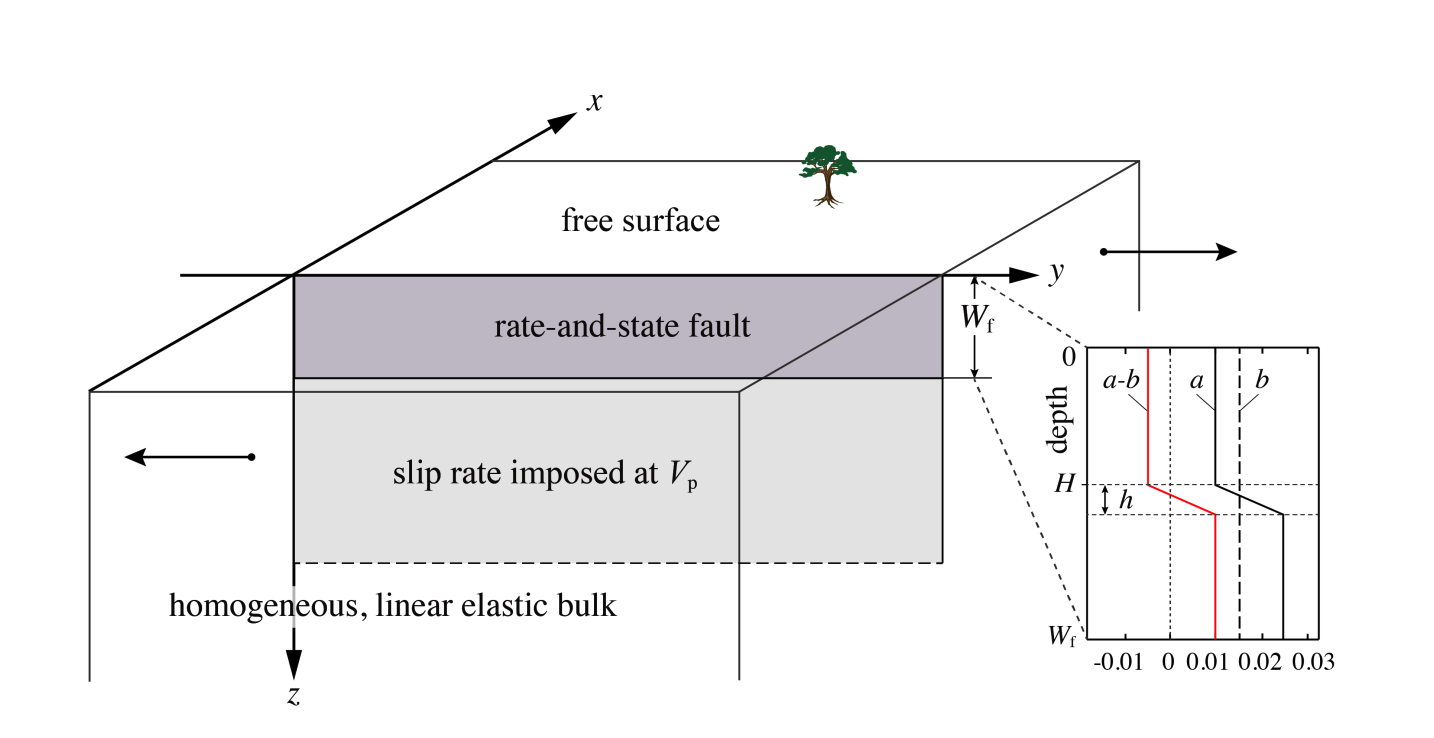
\includegraphics[width=\linewidth]{figures/BP1-figure}
    \caption{BP1 considers a planar fault embedded in a homogeneous, linear elastic halfspace with a free surface. The fault is governed by rate-and-state friction down to the depth $W_f$ and creeps at an imposed constant rate $V_p$ down to the infinite depth. The simulations will include the nucleation, propagation, and arrest of earthquakes, and aseismic slip in the post- and inter-seismic periods. The figure and the description are given in \cite{erickson2018seas}}
    \label{fig:enter-label}
\end{figure}

The problem has a medium size of 401 grid points in each direction after discretization on a 2D domain with around 160k unknowns. 
The conjugate gradient method without a preconditioner on GPUs is fast enough for the simulation to be complete in $\sim$ 2 days on a V100 GPU after solving linear system $\sim$ 300000 times.
It takes around 0.5 seconds to solve linear systems, updating values, and other data operations.
The results for this simulation are published in \cite{erickson2023incorporating} under the model name Thrase.


\begin{figure}
    \centering
    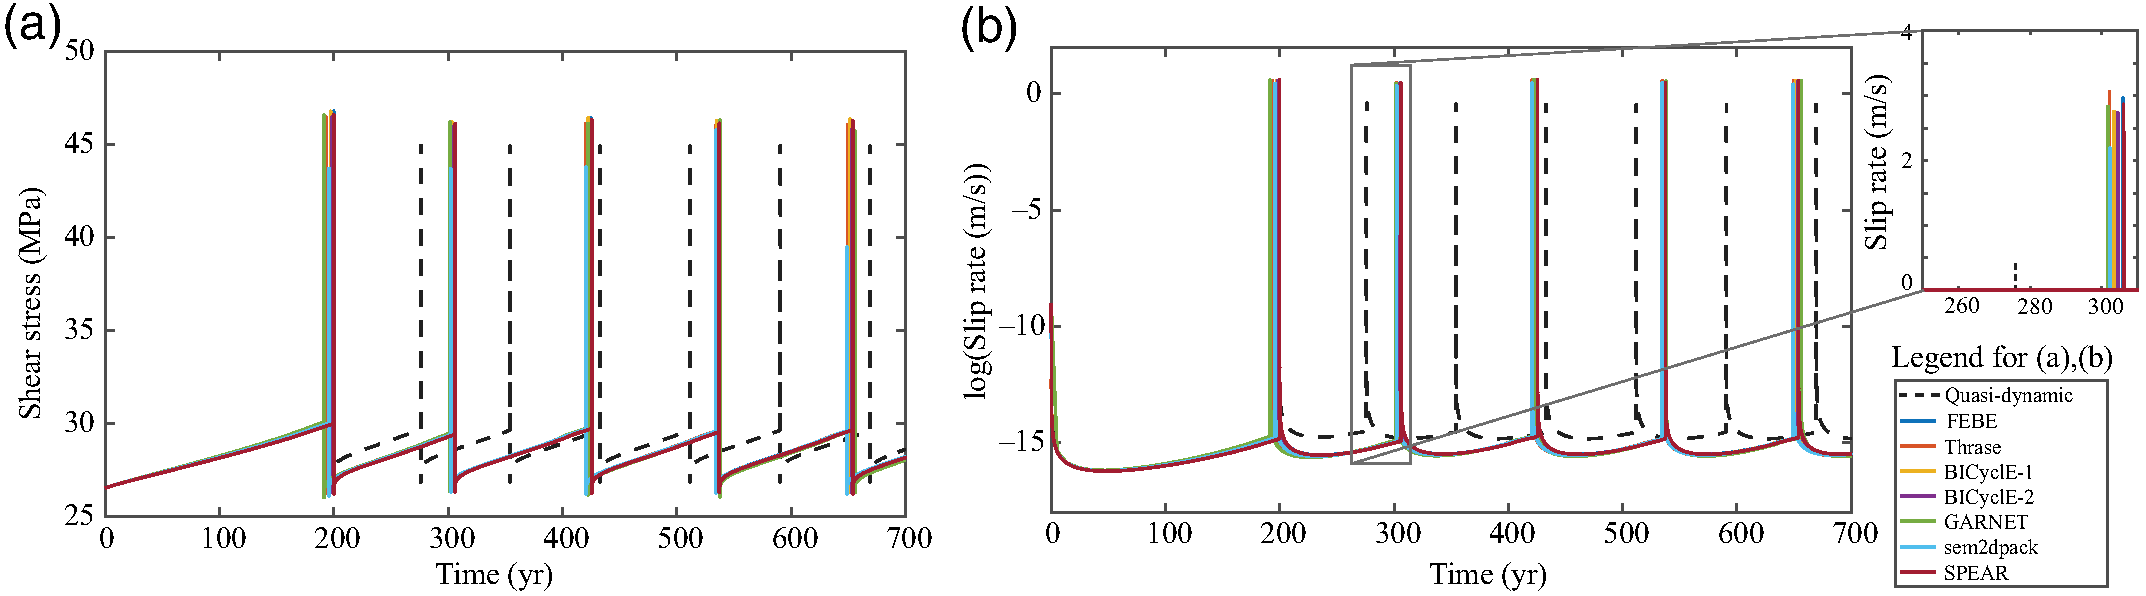
\includegraphics[width=\linewidth]{figures/BP1-seismic-plot.png}
    \caption{Long‐term behavior of BP1‐FD models. Our model name is Thrase in this figure. (a) Shear stress and (b) slip rates at the depth of 7.5 km across codes with sufficiently large computational domain sizes. Also shown (in dashed black) are those for the quasi‐dynamic counterpart BP1‐QD. The color version of this figure is available only in the electronic edition. \cite{erickson2023incorporating}}
    \label{fig:BP1-seismic-plot}
\end{figure}


For the 2D problem with more than 1000 grid point in each direction or a 3D problem with recommended resolutions from benchmark problem 5, we will be solving linear systems with millions or tens of millions of unknowns.
The above approach is too slow even on the latest GPUs.
We need more advanced algorithms like the MGCG method described in Chapter 5.
